\subsection{Basic Algorithm}

The basic algorithm will be to connect interested peers with one another via a DHT that stores peers lists, and the peers themselves will become part of the DHT.  They will store only peer information on the DHT, not blocks themselves.

In our protocol, a peer first tries to download the file from an origin web server.  If at some point one of the following conditions occurs, the download switches to a peer-to-peer swarming download:
\begin{enumerate}
\item First, the client waits a maximum number of seconds $T$ after the start of a normal HTTP download to receive the first byte of data.  If $T$ seconds passes without receiving any data, it transitions to P2P download.  This allows the system to decide quickly whether the origin server is over-burdened and switch to peer-to-peer if needed.   
\item Once the client receives some data from the server, it monitors whether the receive rate falls below a certain fixed threshold of $R$ bytes per second over the last $W$ seconds.  If the receive rate ever drops below $R$, the client switches to peer-to-peer delivery.  This is to accomodate for servers with slow connections or file downloads that become suddenly slow mid-download.
\end{enumerate}

Should the client decide to switch to peer-to-peer delivery, it may need to first lookup meta-data about the file (for example, the size) if it hasn't received any information about the file.  To do so the client calculates a hash value for the URI being download, and looks that up as a $key$ value in the DHT to retrieve a list of meta-data stored there by other peers.  After this, the peers chooses $b$ blocks of the file to download, and retrieves lists of peers who have those blocks by hashing the URI plus the block number, once per block.  The peer selects one peer per block, contacts the peer and requests the block.  After downloading, it then adds itself to the list of peers willing to share that block (see Fig. \ref{fig:download_all_steps}).  While it is attempting to enumerate peers for a block, it connects back to the origin server and requests the block, as well, to not have wasted any time if no peers are found.  If a peer downloads a file whose meta-data is not listed in the DHT, it adds that meta-data to the DHT (for instance, the very first time a peer downloads a file, it will notice that it isn't listed in the DHT and upload meta data for it).  To combat the ``slow last block'' problem,  peers download the last block from several peers simultaneously, similar to BitTorrent \footnote{In reality, we always download from $b$ peers at a time, including for the last blocks, i.e. if you have $b$ set to 10 and have 5 blocks left, each will be downloaded by 2 peers redundantly, and so on down to the last block being downloaded by 10 peers redundantly.}.

\begin{figure*}
  \begin{center}
    \subfigure[Peer downloads list of blocks]{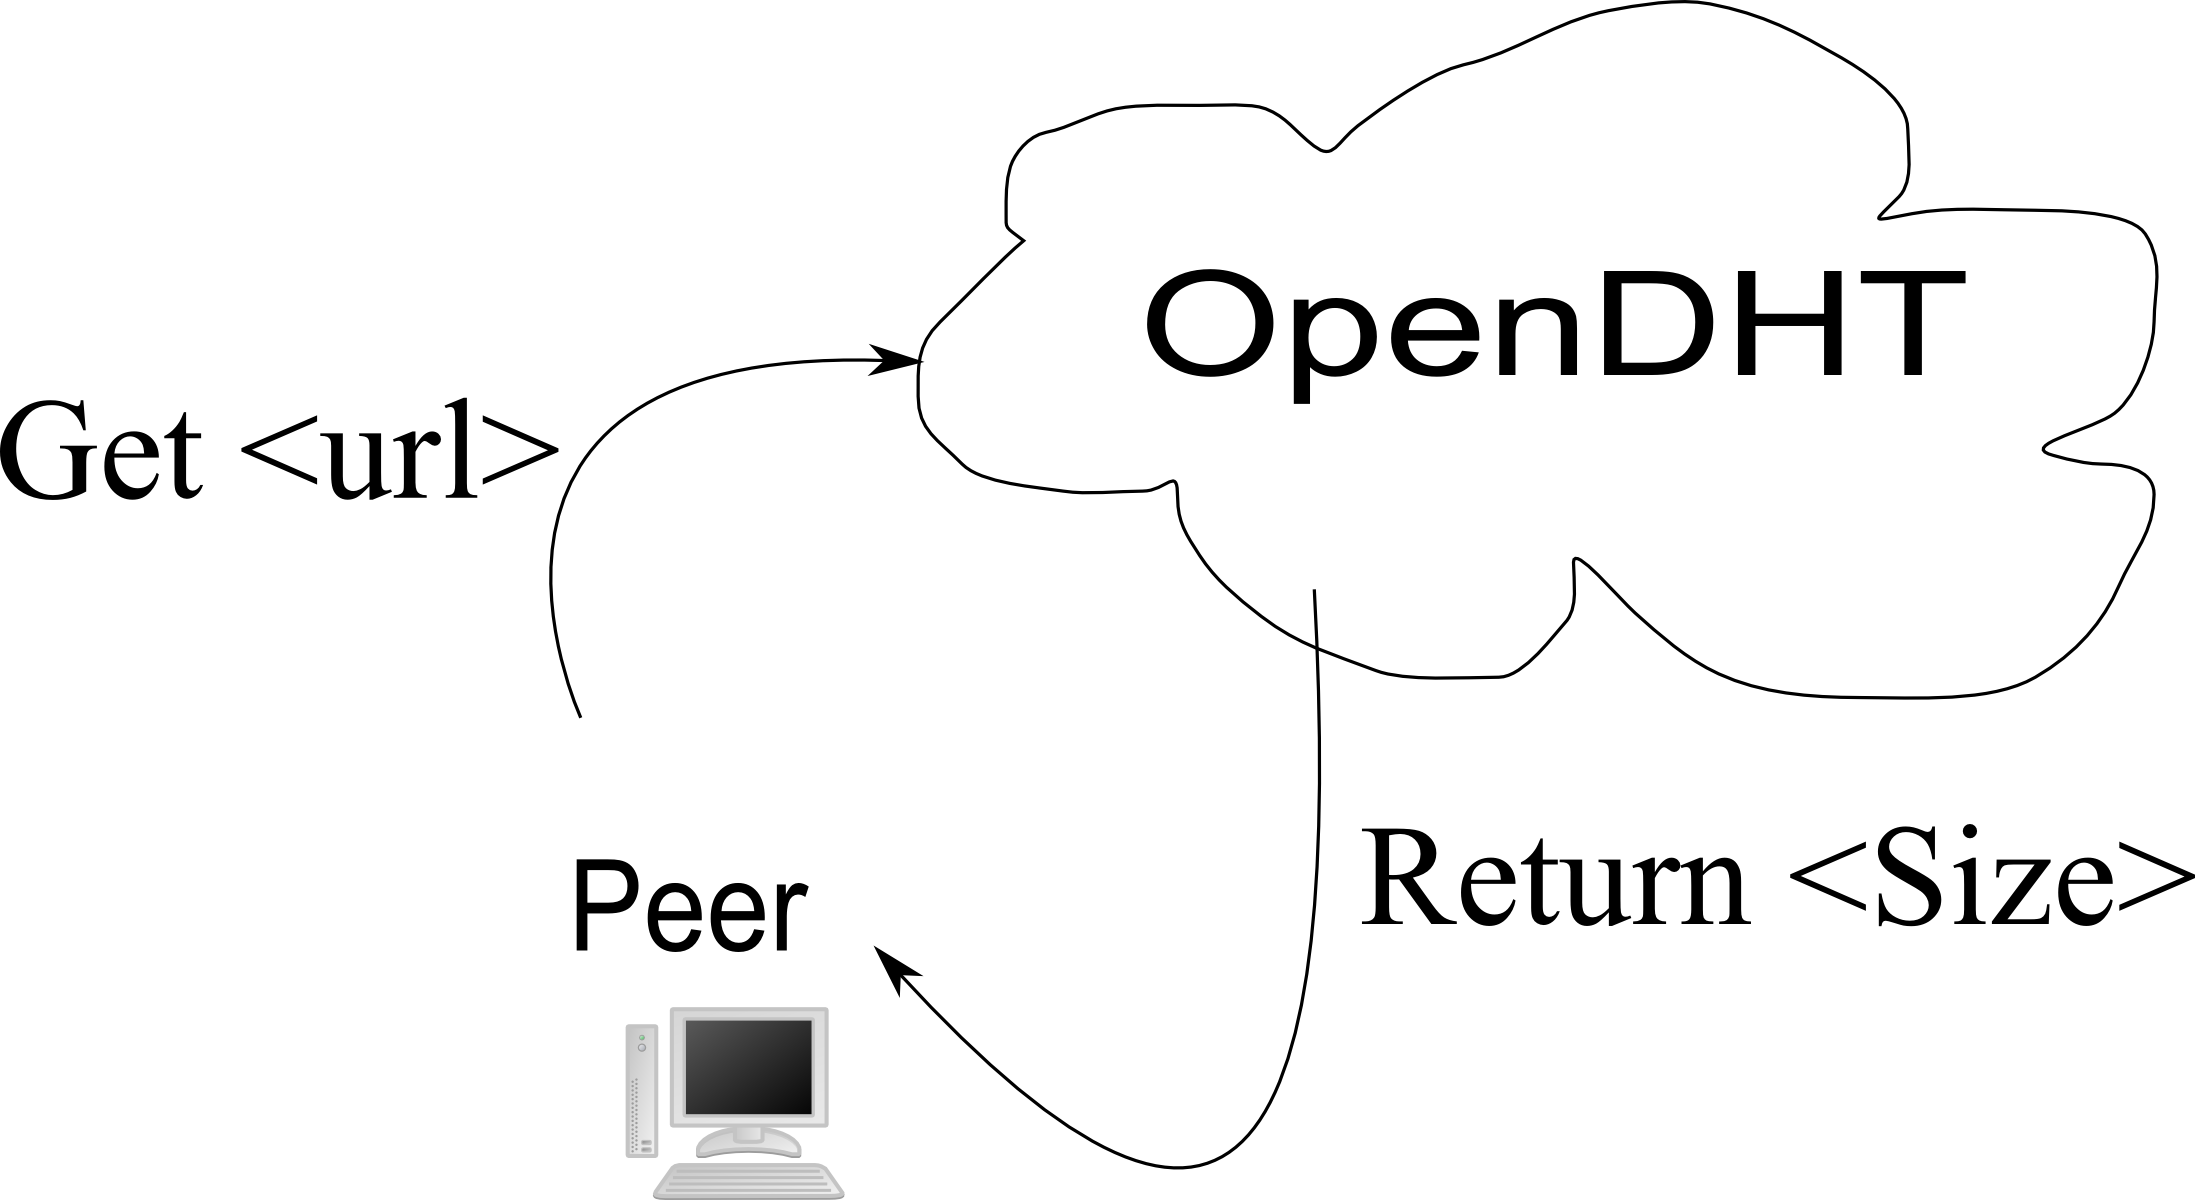
\includegraphics[width=7cm]{description_pics/peer_step_1.png}}
    \subfigure[Peer downloads a list of peers which have a block]{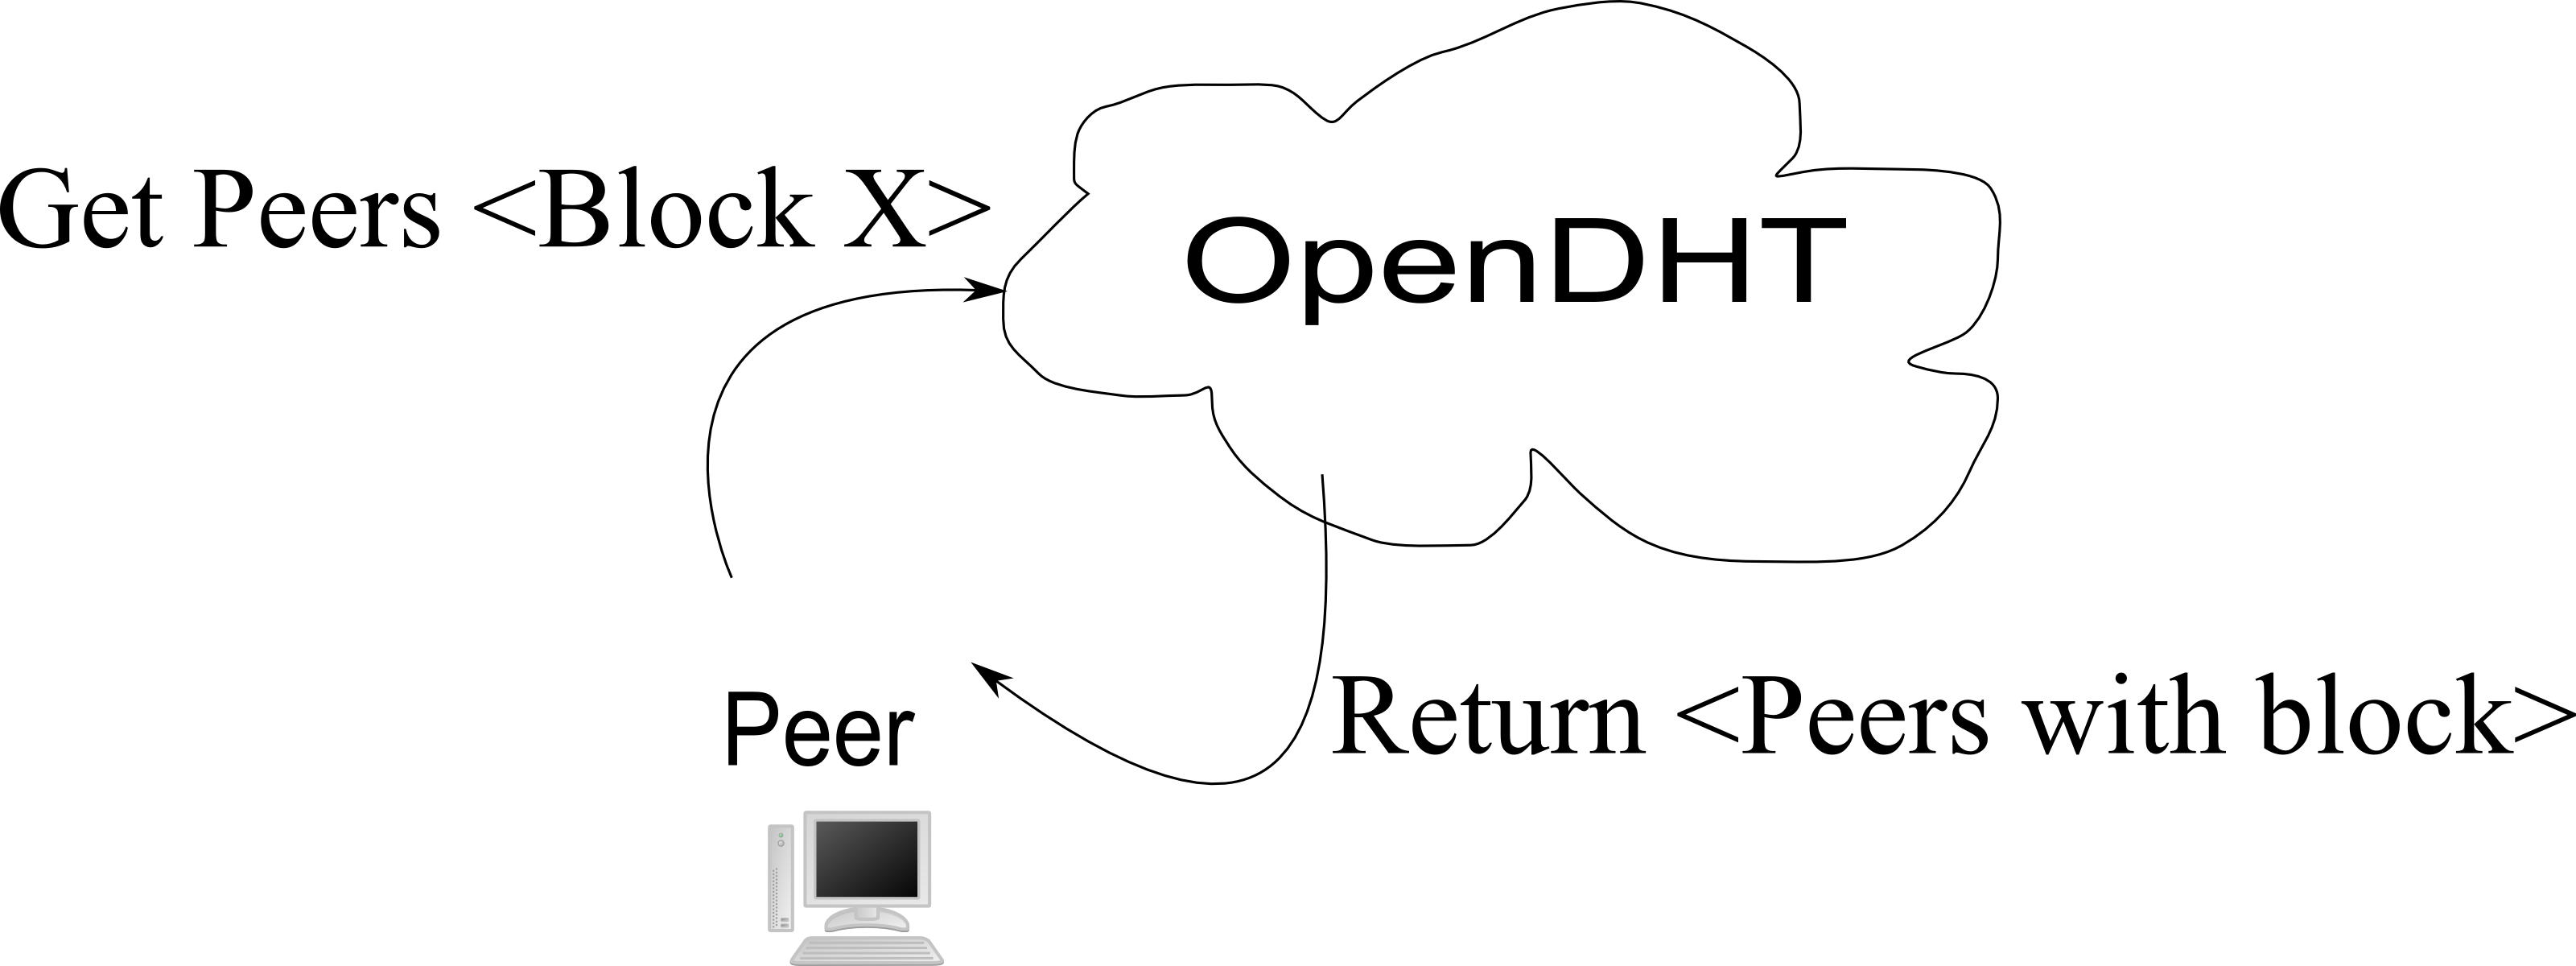
\includegraphics[width=7cm]{description_pics/peer_step_2.png}}
    \subfigure[Peer adds itself to list of peers who have that block]{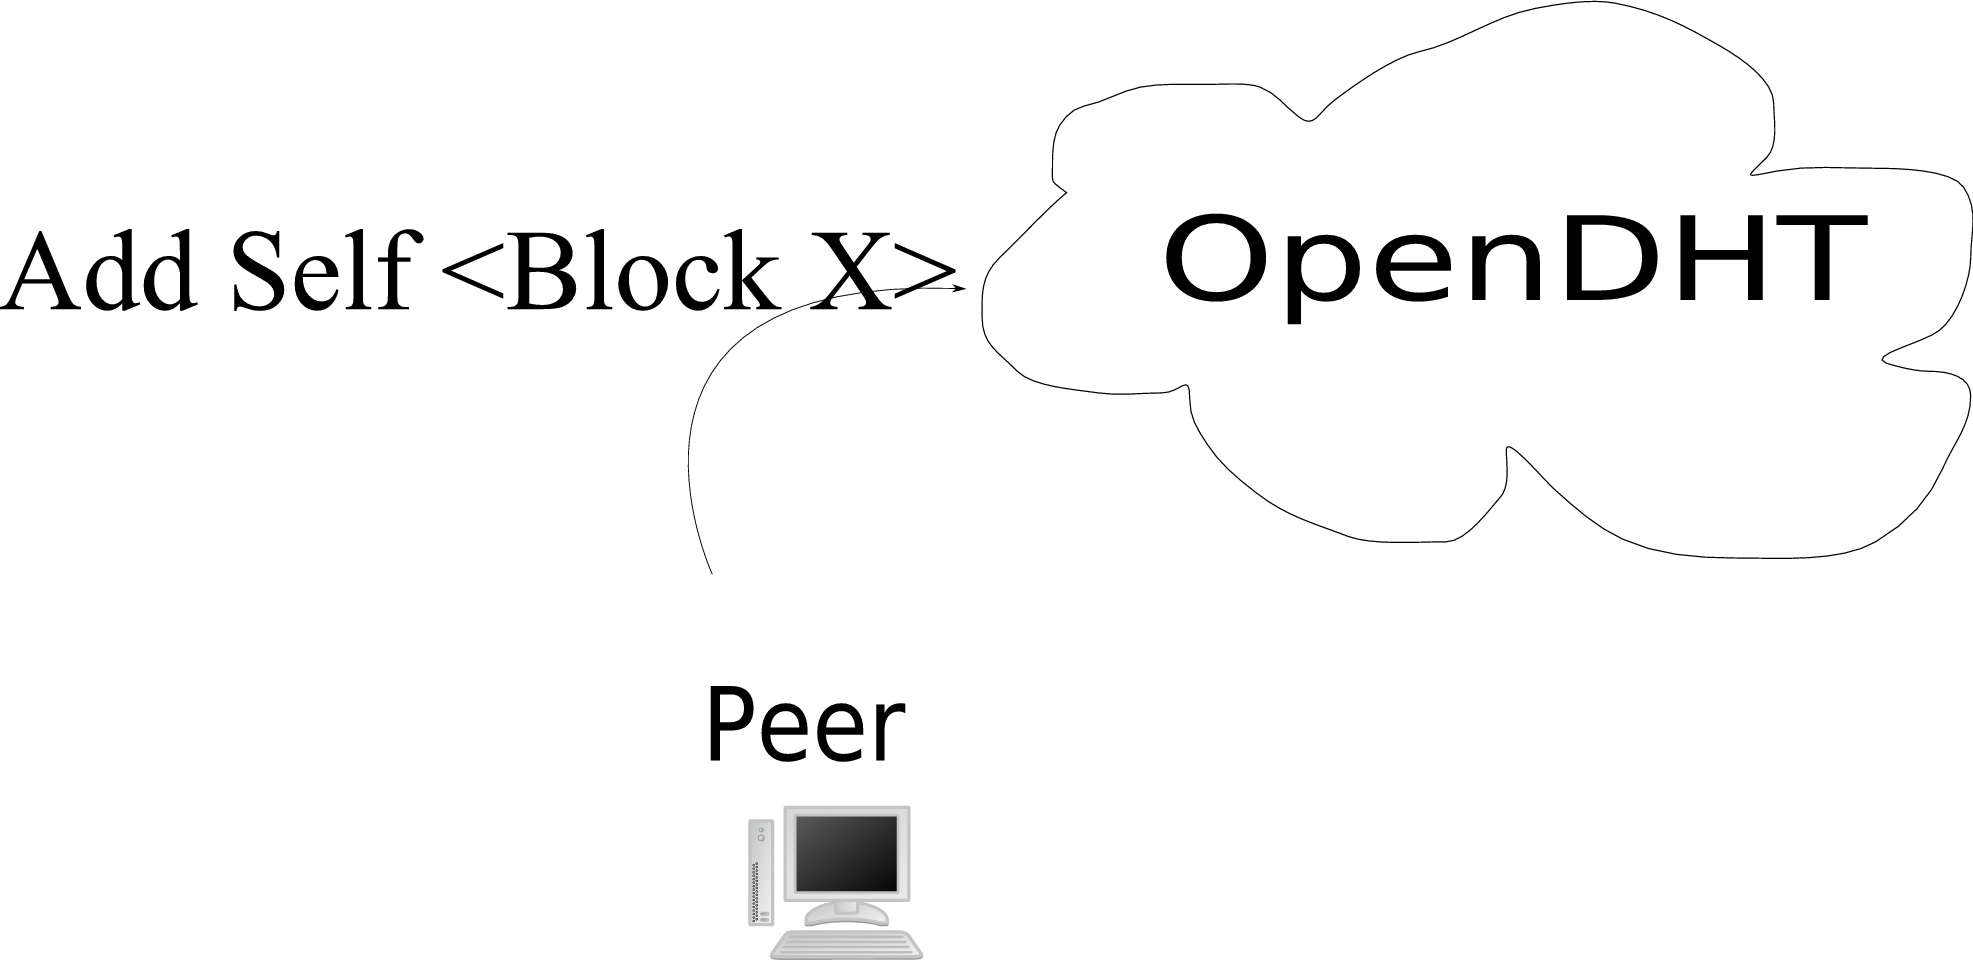
\includegraphics[width=7cm]{description_pics/peer_step_3.png}}
    \caption{Steps to accomplish a peer-to-peer-web download.}
    \label{fig:download_all_steps}
  \end{center}
\end{figure*}

